\documentclass[12pt]{article}
%Gummi|065|=)
\usepackage{amsmath, amsfonts, amssymb}
\usepackage[margin=0.5in]{geometry}
\usepackage{xcolor}
\usepackage{graphicx}

\newcommand{\off}[1]{}
\DeclareMathSizes{20}{30}{20}{18}

\newcommand{\two }{\sqrt[3]{2}}
\newcommand{\four}{\sqrt[3]{4}}
\newcommand{\red}{\begin{tikz}[scale=0.25]
\draw[fill=red, color=red] (0,0)--(1,0)--(1,1)--(0,1)--cycle;\end{tikz}}
\newcommand{\blue}{\begin{tikz}[scale=0.25]
\draw[fill=blue, color=blue] (0,0)--(1,0)--(1,1)--(0,1)--cycle;\end{tikz}}
\newcommand{\green}{\begin{tikz}[scale=0.25]
\draw[fill=green, color=green] (0,0)--(1,0)--(1,1)--(0,1)--cycle;\end{tikz}}

\newcommand{\sq}[3]{\draw[#3] (#1,#2)--(#1+1,#2)--(#1+1,#2+1)--(#1,#2+1)--cycle;}

\usepackage{tikz}

\newcommand{\susy}{{\bf Q}}
\newcommand{\RV}{{\text{R}_\text{V}}}

\title{Worksheet: Exotic Number Systems}
\author{John D Mangual}
\date{}
\begin{document}

\fontfamily{qag}\selectfont \fontsize{12.5}{15}\selectfont

\maketitle

\noindent Something truly exotic challenges your norms a little bit\dots makes one feel uneasy. \\ \\
The goal of this project is to study new numbers and number-like things.  We only try a small fraction of the ideas available. And there's no guarantee this will work. \\ \\
Our decimal system is intimately related to the multiplication by ten shift map $\times 10$ we can envision a number as a sequence of decimal digits (kind of like a factory)
$$ \pi = 3. \to  1 \to 4 \to 1 \to 5 \to 9 \to \dots $$
Each digit is connected to the last by one either by multplying by ten or shifting by 1:
\begin{itemize}
\item $T: x \mapsto (10 \times x ) \pmod 1 $  with  $x \in \mathbb{R}$\\ 
\item $T: (x_0, x_1, x_2, \dots ) \mapsto (x_1, x_2, x_3, \dots ) $ with $x \in \{0,1\}^\mathbb{N}$
\end{itemize}
This framework kind of forgets that $\mathbb{R}$ is a ring $(\mathbb{R}, + , \times)$ or even a group $(\mathbb{R}, +)$.  Regardless of our choice of $T$ we can say that rings are isomorphic. Yet, in reality we must make a choice of $T$, and it can have nothing to do with the decimal system.
$$ (x_0, x_1, x_2, \dots ) \oplus (y_0, y_1, y_2, \dots ) = \;? $$
Our goal is to explain the different ways $\mathbb{R}$ could be partitioned and try to achieve an analogue of addition with carries.  Some partitions are more ordinary, others are more unique. 

\newpage

\noindent \textbf{6/15} I have a lot on my mind.  I saw a discussion on the internet that made me re-think all the proofs I could think of about the irrationality of $\sqrt{2}$.  Wikipedia suggested that descent proofs like this one:
$$ p^2 = 2q^2 \to p \equiv 0 \pmod 2 \to p = 2r \to (2r)^2 = 2q^2 \to q^2 = 2r^2  $$
are examples of Galois cohomology.  Is that true? Textbooks other than Wikipedia use another example:
$$ p = a^2 + b^2 \quad\text{ iff}\quad p = 4k+1 $$
Unfortunately, none of these textbooks explain how to simplify the machinery or to build it from scratch.   I even went as far as to ask the very authors of the textbooks themselves, and they didn't know, they didn't care; they have bigger fish to fry. \\ \\
They really do.  I do not.  \\ \\
This is how I learn and teach: agonizing over the basics attaching names to everything. Their theory is failing my textcase, and these days I'd rather believe my own experience than 100 experts.\\ \\
Intermediate between elementary number theory.  Is the theory of \textbf{heights}.  On the set of pairs fractions or pairs of integers we could assign a number:
$$ \bigg[ \frac{p}{q} \in \mathbb{Q} \bigg] \leftrightarrow  \bigg[ [p:q] \in \mathbb{Q}P^1 \bigg] \mapsto |p|+|q| \in \mathbb{Z} \subset \mathbb{R} $$
The map $(p,q) \mapsto (q,r)$ leads to an infinite decreasing sequence of heights with values in $\mathbb{Z}_{\geq 0}$ which is impossible.  \\ \\
Then we find out height are related to \textbf{torsors} which are then related to a cohomology of some kind.  I am scared there will be other examples of instances of heights that are not so trivial, and I will be unable. \\ \\
There are textbooks on Galois Cohomology written by smart guys like JP Serre who give outlines, but in a way we're on our own.  Even the cohomology theory we could build ourselves. \\ \\
Why such a complicated thing?  I could total envision an arithmetic where our fractions:
$$ \bigg[ \frac{p}{q} \in \mathbb{Q} \bigg] $$
Our replaced with some other complicated figment of our imagination, which may also prove to be a useful arithemtic concept.  Our goal is to solve the equation:
$$  \bigg\{  x^2 - 2y^2 = 0 \bigg\} \stackrel{?}{=} [\varnothing ]\subseteq \mathbb{Q}^2  $$
How can this equation be nothing it is the union of two lines.  Clearly I can re-write this as:
$$ x^2 - 2y^2 = (x-\sqrt{2}y) ( x + \sqrt{2}y) = 0 \text{ therefore } \Big[ x-\sqrt{2}y = 0\Big] \text{ or }
\Big[ x+\sqrt{2}y = 0 \Big] $$
Is this OK?  And if not, there are 28 other proofs I can find on the internet\footnote{\texttt{http://www.cut-the-knot.org/proofs/sq\_{}root.shtml}}

\newpage

\noindent \textbf{6/19} The best way I can think of to run through the ``higher algebra" content of irrationality proofs is to do one. \\ \\
cut-the-knot.com Proof \#8 involves patchwork of square.  Literally $x^2 = 2y^2$ looks like this:
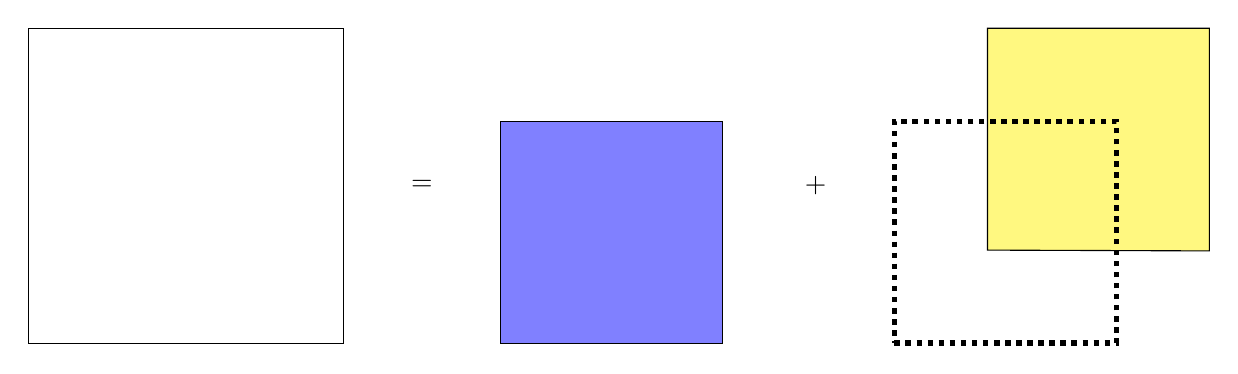
\begin{tikzpicture}
\draw(0,0)--(4,0)--(4,4)--(0,4)--cycle;

\begin{scope}[xshift=6cm]
\draw[fill=blue!50!white] (0,0)--(2.818,0)--(2.818,2.818)--(0,2.818)--cycle;
\end{scope}

\begin{scope}[xshift=11cm]

\draw[fill=yellow!50!white] (4-2.818,4-2.818)--(4-2.818+ 2.818,4-2.828)--(4-2.818+ 2.818,4)--(4-2.818,4)--cycle;
\draw[dotted, line width = 2] (0,0)--(2.818,0)--(2.818,2.818)--(0,2.818)--cycle;
\end{scope}

\node at (10,2) {$+$};
\node at (5,2) {$=$};
\end{tikzpicture} \\ 
Literally, these squares can be considered the second homology of the plane, $H_2(\mathbb{R}^2)$. \\
If we superimpose the three squares as shown: \\ \\
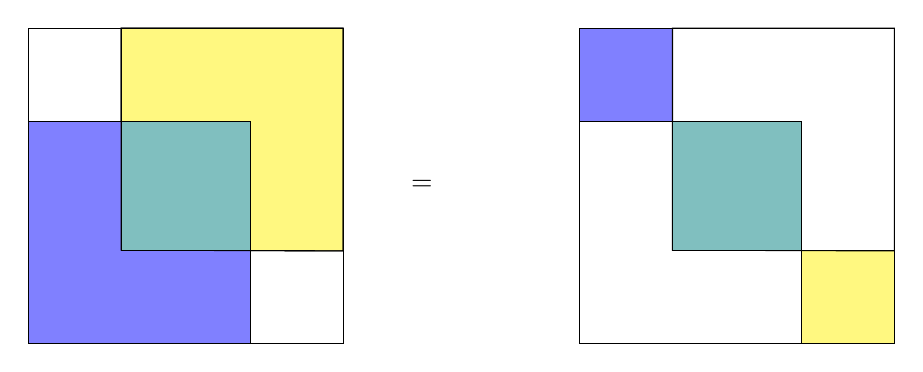
\begin{tikzpicture}
\draw(0,0)--(4,0)--(4,4)--(0,4)--cycle;

\draw[fill=yellow!50!white] (4-2.818,4-2.818)--(4,4-2.828)--(4,4)--(4-2.818,4)--cycle;
\draw[fill=blue!50!white] (0,0)--(2.818,0)--(2.818,2.818)--(0,2.818)--cycle;
\draw (0,0)--(2.818,0)--(2.818,2.818)--(0,2.818)--cycle;

\draw (4-2.818,4-2.818)--(4,4-2.828)--(4,4)--(4-2.818,4)--cycle;

\draw[fill=green!50!blue!50!white] (4-2.818,4-2.818)--(2.818,4-2.818)--(2.818, 2.818)--(4-2.818,2.818)--cycle;


\begin{scope}[xshift=7cm]

\draw(0,0)--(4,0)--(4,4)--(0,4)--cycle;

\draw[fill=yellow!50!white] (2.818,0)--(4,0)--(4,4-2.818)--(2.818,4-2.818)--cycle;

\draw[fill=blue!50!white] (0,2.818)--(4-2.818,2.818)--(4-2.818,4)--(0,4)--cycle;

\draw (0,0)--(2.818,0)--(2.818,2.818)--(0,2.818)--cycle;

\draw (4-2.818,4-2.818)--(4,4-2.828)--(4,4)--(4-2.818,4)--cycle;

\draw[fill=green!50!blue!50!white] (4-2.818,4-2.818)--(2.818,4-2.818)--(2.818, 2.818)--(4-2.818,2.818)--cycle;

\end{scope}

\node at (5,2) {$=$};

\end{tikzpicture} \\ \\ 
By the \textbf{Carpets Theorem} (stated without proof), the area of the blue and yellow squares totals to the area of the green square.  The blue and yellow squares have the same area. \\
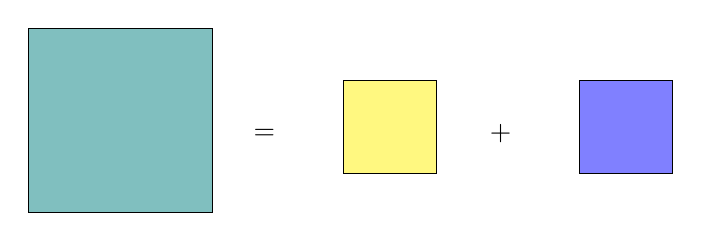
\begin{tikzpicture}
\draw[fill=green!50!blue!50!white](0,0)--( 4*2 - 4*1.414,0)--( 4*2 - 4*1.414,4*2 - 4*1.414)--( 0,4*2 - 4*1.414)--cycle;

\begin{scope}[xshift=4cm, yshift=0.5cm]
\draw[fill=yellow!50!white] (0,0)--(4-2.818,0)--(4-2.818,4-2.818)--(0,4-2.818)--cycle;
\end{scope}

\begin{scope}[xshift=7cm, yshift=0.5cm]
\draw[fill=blue!50!white] (0,0)--(4-2.818,0)--(4-2.818,4-2.818)--(0,4-2.818)--cycle;
\end{scope}

\node at (6,1) {$+$};
\node at (3,1) {$=$};
\end{tikzpicture} \\ 
We continue to overthink the situation:
\begin{itemize}
\item $
\text{Area} (\begin{tikz}\draw(0,0)--(10pt,0)--(10pt,10pt)--(0,10pt)--cycle;\end{tikz} )
- \Big( \text{Area}( \begin{tikz}\draw[fill=yellow!50!white](0,0)--(10pt,0)--(10pt,10pt)--(0,10pt)--cycle;\end{tikz})
+ \text{Area}(\begin{tikz}\draw[fill=blue!50!white](0,0)--(10pt,0)--(10pt,10pt)--(0,10pt)--cycle;\end{tikz}) \Big) - \text{Area}(\begin{tikz}\draw[fill=blue!50!green!50!white](0,0)--(10pt,0)--(10pt,10pt)--(0,10pt)--cycle;\end{tikz})  = 0 $ the \textbf{inclusion-exclusion} principle
\item $
\text{Area}( \begin{tikz}\draw[fill=yellow!50!white](0,0)--(10pt,0)--(10pt,10pt)--(0,10pt)--cycle;\end{tikz})
= \;\;\text{Area}(\begin{tikz}\draw[fill=blue!50!white](0,0)--(10pt,0)--(10pt,10pt)--(0,10pt)--cycle;\end{tikz}) $ \hspace{2.11in} symmetry
\end{itemize}
If you know a little bit of programming you might try to understand the area-conservation statement here.\footnote{\texttt{http://www.cut-the-knot.org/Curriculum/Geometry/CarpetsInSquare.shtml}} In my case, I prefer the programmig language \textsc{\textbf{Elm}}.  Obviously you are welcome to use anything you like. \\ \\
If we tried to write this purely in terms of Algebra:
$$ X \otimes X = A \otimes A + B \otimes B  $$
The only other parameter I can think of is the amount of intersection of $\square_A \cap \square_B$:
$$  X = A + B - C $$
If I pursue this and try to take the tensor product:
\begin{eqnarray*} X \otimes X &=& (A + B - C) \otimes (A + B - C) \\  
&=& A \otimes A + B \otimes B + C \otimes C \\
&+& \big( A \otimes B + B \otimes A\big)
- \big( B \otimes C + C \otimes B\big)
- \big( C \otimes A + A \otimes C\big) \end{eqnarray*}
Judging from the diagrams I can write another set of areas:
\begin{eqnarray*}
0 &=& (-1)(X-A) \otimes (X-A) + (-1)(X-B) \otimes (X-B) +
\Big( 2\,X - (A+B) \Big)\otimes \Big(2\,X - (A+B)\Big) \end{eqnarray*}
Not totally sure right now.  The carpets theorem enable to turn one diagram into the other:
$$ A \mapsto X - A \hspace{0.5in} B \mapsto X-B 
\hspace{0.5in} C \mapsto (X-A+X-B)-X$$
and the statements about areas in one equations, turn into the second equation.  These could be statemets in $\mathbb{H}_2 (\mathbb{R})$.  The implication is something like:
$$ \bigg[ \;\; X^2 = A^2 + B^2 \;\; \bigg] \to \Bigg[\;\; (X-A)^2 + (X-B)^2 = (2X - A - B)^2 \;\; \Bigg] $$
In fact, these are not equal.  These two are off by a certain amount:
$$ 2 \,\big( X^2 - AX - BX + AB \big) = 2 \,(X-A)\,(X-B) $$
One issue, is the small blue and yellow have equal area.  In our algebra we'd need $A = B$.  Or maybe they're not quite the same, but as segments in the plane: $ A \simeq B \in H_1(\mathbb{R}^2$). \\ \\
These ideas need lots of refining, but \textbf{Euclidean geometry} = (trivial) \textbf{Homology of the Euclidean Plane}.  And there is non-trivial homology as well.

\newpage

\noindent \textbf{6/20} We move into uncharted. Territory.  Carlos and I have had exchanges online, but I don't know him or anything.  They seem to be really good at Dynamics in Brazil.  \\ \\
Dynamics here $\neq$ Dynamics on Homogenous spaces; \\ \\
These could be iterations of polynomials, or evolutions of differential equations.  Bifurcations and more. \\ \\
One of his latest blogs he reviews the \textbf{Markov spectrum} and \textbf{Lagrange spectrum}.   If we rewind to 2009, he has already reviewed what they are.\footnote{\texttt{https://matheuscmss.wordpress.com/2009/07/30/gugus-theorem-on-the-markov-and-lagrange-spectrum/}} Lagrange's Theorem says:
$$ \Big| \Big\{ \frac{p}{q}:  \big|  \alpha - \frac{p}{q} \big| < \frac{1}{q^2} \Big\} \Big| = \infty $$
This inequality seems OK. \\ \\
In my mind, I always thought all fractions were kind of the same.  If we write them with decials they look very even:
$$ 0.0 < 0.1 < 0.2 < 0.3 < \textbf{0.31} < \textbf{0.32} < \textbf{0.33} < \dots < 
\textbf{0.39} < 0.4 < 0.5 < 0.6 < 0.7 < 0.8 < 0.9 < 1.0 $$
If we look at fractions by denominator, the spread is telling a very different story:
$$  0 < \frac{1}{5} < \frac{1}{4} <   \frac{1}{3} < \frac{2}{5} <  \frac{1}{2} < \frac{3}{5} < \frac{2}{3}  < \frac{3}{4} <  \frac{4}{5} < 1  $$
There are lots of approximations to irrational numbers that are particularly fast.  One can solve:
$$ \Big|  \alpha - \frac{p}{q} \Big| < \frac{1}{q^2}  $$
but we can do even better by a factor of $\sqrt{5}$ for any $\alpha$. Then it stops. 
$$ \Big|  \alpha - \frac{p}{q} \Big| <  \;\frac{1}{\sqrt{5}}\;\frac{1}{q^2}  $$
The next bext constant I believe is $2 \sqrt{2}$.  There exist irrational numbers such that:
$$\Big|  \alpha - \frac{p}{q} \Big| <  \;\frac{1}{2\sqrt{2}}\;\frac{1}{q^2}  $$
and the next best number after that is $\sqrt{221}/5$.  And there are infinitely many of those\dots \\ \\
There is a whole Lagrange spectrum:
$$ k (\alpha) := \sup \bigg\{ k > 0 : \Big| \alpha - \frac{p}{q} \Big| < \frac{1}{k \, q^2}  \bigg\} \hspace{0.25in}\text{and}\hspace{0.25in} L = \big\{ k(\alpha): \alpha \in \mathbb{R} - \mathbb{Q}, k(\alpha) < \infty \big\}  $$
This definition is rather complicated, and as we move further along the Lagrange spectrum, these numbers are getting rather weird or specific.

\newpage

\noindent Carlos Matheus is really smart guy.  I can already tell\dots  he's going to tell us about the Lagrange spectrum but not necessarily the numbers that exhibit them. We know that: 
$$ \mu \big( \alpha \in \mathbb{R} : k(\alpha) = \infty \big) = 1 $$
This is a hard formula to interpret.  For basically \textbf{all} numbers we can get really good continued fraction approximations.  The Lagrange spectrum measures the exceptions.  And it has a weird, not-totally-understood shape.\\ \\
We're not going to fully comprehend it either.  Instead, there will be room for us to do action. Can  you name an $\alpha \in \mathbb{R}$ such that:
$$ \# \bigg\{ \frac{p}{q} \in \mathbb{Q} : \Big|  \alpha - \frac{p}{q} \Big| <  \;\frac{1}{2\sqrt{2}}\;\frac{1}{q^2} \bigg\} \stackrel{?}{=} \infty $$
He will reason about a lot of Cantor sets, that I would like to draw.  He won't. A priori, this may not the best approach.  \\ \\
I am a little bit nervious that $[6, +\infty) \subset L$.  This is basically the whole real number line to the right of 6 is part of Lagrange spectrum.  We know all there are a bunch of dots to the left of 3.   \\ \\
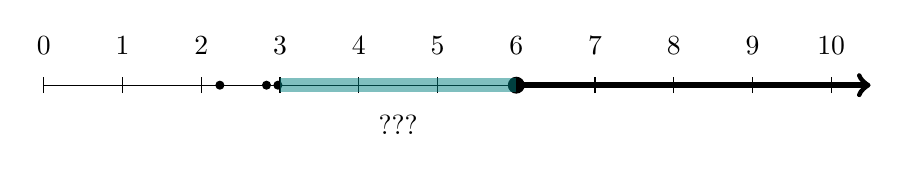
\begin{tikzpicture}

\draw (0,0)--(10,0);
\foreach \a in {0,...,10}{
	\draw (\a,-0.1)--(\a,0.1);
	\node at (\a,0.5) {\a};	
}

\draw[fill=black] (6,0) circle (0.1);
\draw[line width = 2, ->] (6,0)--(10.5,0);

\draw[fill=black] (2.236,0) circle (0.05);
\draw[fill=black] (2.828,0) circle (0.05);
\draw[fill=black] (2.973,0) circle (0.05);

\draw[line width = 5, , opacity=0.5, color=green!50!blue] (3,0)--(6,0);

\node at (4.5,-0.5) {???};
\end{tikzpicture} \\ 
In between 3 and 6 we know absolutely nothing.  Carlos' friend Gugu will show us a thing or two about these exotic numbers.

\vfill 

\begin{thebibliography}{}

\item Michael Baake, Natalie Frank , Uwe Grimm , E. Arthur Robinson 
\textbf{Geometric properties of a binary non-Pisot inflation and absence of absolutely continuous diffraction} \texttt{arXiv:1706.03976} 

\item Roy L. Adler.  \textbf{Symbolic dynamics and Markov partitions}

Bull. Amer. Math. Soc. 35 (1998), 1-56 

\item Carlos Matheus \textbf{New Numbers in M-L}\\ \texttt{https://matheuscmss.wordpress.com/2017/04/05/new-numbers-in-m-l/}

\end{thebibliography}


\end{document}